\documentclass[12pt]{article}
\usepackage[hmargin={1in},vmargin={.95in,.85in},foot={.6in}]{geometry}   
\geometry{letterpaper}       
%\geometry{landscape}          
%\usepackage[parfill]{parskip}
\usepackage{color,graphicx}
%\usepackage{covington}
%\usepackage{xyling}
\usepackage{setspace}
\usepackage{amsmath}
\usepackage{amssymb}
%\usepackage{graphicx,color}
%\usepackage{theorem}
%\usepackage{tabularx}
%\usepackage{subfig}
%\usepackage{vowel}
%\usepackage{mathrsfs}
\usepackage{varioref}
\usepackage{textcomp}
%\usepackage{avm}
\usepackage{textcomp}
\usepackage{mflogo}
\usepackage{wasysym}
%\usepackage{pstricks, pst-plot, pst-node, pst-tree, colortab}
%\usepackage{qtree}
 %\usepackage{tree-dvips}
 \usepackage{linguex}
%\usepackage{gb4e}
 \usepackage{multirow}
 %\usepackage[stable]{footmisc}
 \usepackage{pifont}
%\usepackage{todonotes}
\usepackage{natbib}
\usepackage[normalem]{ulem}
\usepackage{wrapfig}

 %\setlength{\parskip}{.55ex plus 0.1ex}


\usepackage{fancyhdr} % This should be set AFTER setting up the page geometry
\pagestyle{plain} % options: empty , plain , fancy
\lhead{}\chead{}\rhead{}
\renewcommand{\headrulewidth}{.3pt}
\lfoot{}\cfoot{\thepage}\rfoot{}
%\renewcommand{\footrulewidth}{.3pt}
\newcommand{\txtp}{\textipa}
\renewcommand{\rm}{\textrm}
\newcommand{\sem}[1]{\mbox{$[\![$#1$]\!]$}}
\newcommand{\lam}{$\lambda$}
\newcommand{\lan}{$\langle$}
\newcommand{\ran}{$\rangle$}
\newcommand{\type}[1]{\ensuremath{\left \langle #1 \right \rangle }}
\newcommand{\defeq}{$\mathrel{\mathop:}=$ }
\renewcommand{\and}{$\wedge$ }


%\renewcommand{\Extopsep}{2pt}


\newcommand{\bex}{\begin{examples}}
\newcommand{\eex}{\end{examples}}

%bullet points
\newcommand{\bit}{\begin{itemize}}
\newcommand{\eit}{\end{itemize}}

%numbering, non sequential
\newcommand{\ben}{\begin{enumerate}}
\newcommand{\een}{\end{enumerate}}

\renewcommand{\abstractname}{The goal:}


%numbering, what you would use in a paper when you don't want the numbering to stop every time you end an example. 
%\newcommand{\bex}{\begin{enumerate}\setcounter{enumi}{\thesaveenumi}\item{}\begin{enumerate}}
%\newcommand{\eex}{\end{enumerate}\setcounter{saveenumi}{\theenumi}\end{enumerate}}

%%these are the brackets used for writing up semantic meanings 
%\newcommand{\lbr}{\textrm{\textlbrackdbl}}
%\newcommand{\rbr}{\textrm{\textrbrackdbl}}
%\renewcommand{\rm}{\textrm}

%this describes the numbering system (roman vs arabic numerals and so forth)
\renewcommand\theenumi {\alph{enumi}}
\renewcommand\theenumii {\alph{enumii}}
\renewcommand\labelenumi {\theenumi. }
\renewcommand\labelenumii {\theenumii.}
\labelformat{enumi}{(\theenumi)}
\labelformat{enumii}{(\theenumi\theenumii)}
\newcounter{saveenumi}

%\renewcommand{\labelitemi}{\textbf{---}}
%\renewcommand{\labelitemii}{\textbf{$\cdot$}}

%\linespread{1.5}

%\qtreecenterfalse

%\linespread{1}

\begin{document}

\begin{center}\textbf{The role of context in plural predication}\\
	Gregory Scontras and Noah D.\ Goodman --- \emph{Stanford University}\\*[5pt]
\end{center}

\vspace{-11pt}

\noindent Predicates like \textit{heavy} or \textit{expensive} admit both distributive and collective interpretations: \textit{The boxes are heavy} can mean either that each member of some salient set of boxes is heavy (distributive), or that taken together the whole set counts as heavy (collective; \citealp{scha1984}). Since \citet[p.140]{quine1960}, researchers have assumed that some predicates lack collective interpretations: \textit{The boxes are big} is said to communicate about individual, but not total box size. Other size and shape predicates behave similarly (e.g., \emph{long}, \emph{round}); \cite{schwarzschild2011} terms them ``stubbornly distributive.'' To address the issue of why (and whether) these predicates differ, we begin with the more basic question of how much the interpretation of plural predication depends on context, and in what way. The answer may illuminate both the semantics of plural predication and the pragmatic mechanisms of ambiguity resolution. We first establish a way of studying plural predication experimentally. In Expt.~1, we introduce and validate a new paraphrase methodology. We then explore the idea that contextual predictability of the relevant collective property is a critical factor in determining which reading is used. Expt.~2 shows that less variable contexts make the collective more acceptable for all of the predicates tested. Finally, we discuss the role of contextual predictability under a pragmatic account of ambiguity resolution in plural predication, using a Bayesian model to formalize the process.

%Our study identifies the difference between possibly collective and stubbornly distributive predicates as one of potential interpretation noise (noisier interpretations are less useful and thus less likely), and demonstrates that the choice between distributive and collective interpretations depends in part on the quality of the property being predicated, but crucially on the context in which this predication transpires. With the proper context, so-called stubbornly distributive predicates become remarkably compliant.

%Concretely, we show that the probability of an interpretation depends crucially on potential variability in the property being communicated. 

	\begin{wrapfigure}[27]{r}{.5\textwidth}
		\vspace{-33pt}
			\Exlabelsep = 0pt
			\ex. \label{bare} The boxes were big/heavy/tall.
			
			\ex. \label{each} The boxes {each} were big/heavy/tall.
			
			\ex. \label{tog} The boxes {together} were big/heavy/tall.
			
	 	\centering
	 	\vspace{-2pt}
	 	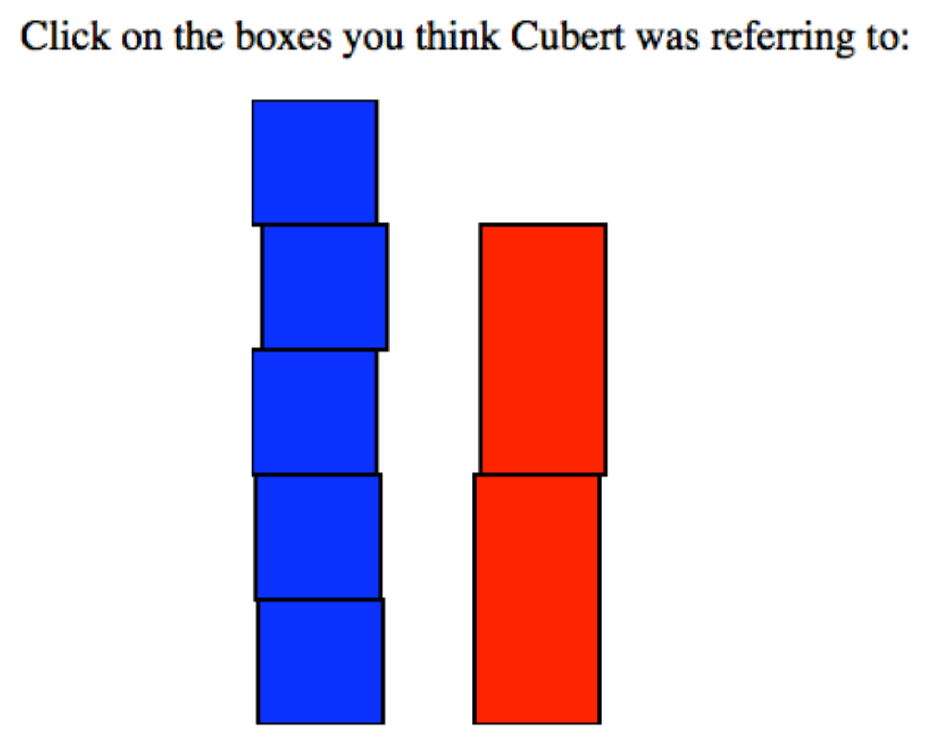
\includegraphics[width=.95\linewidth]{trial2.eps}\\
	 	\vspace{-3pt}
	 	\mbox{Fig.~1: Sample trial from Expt.~1.}\\
	 	%\vspace{-2pt}
	 	\mbox{\hspace{-11pt}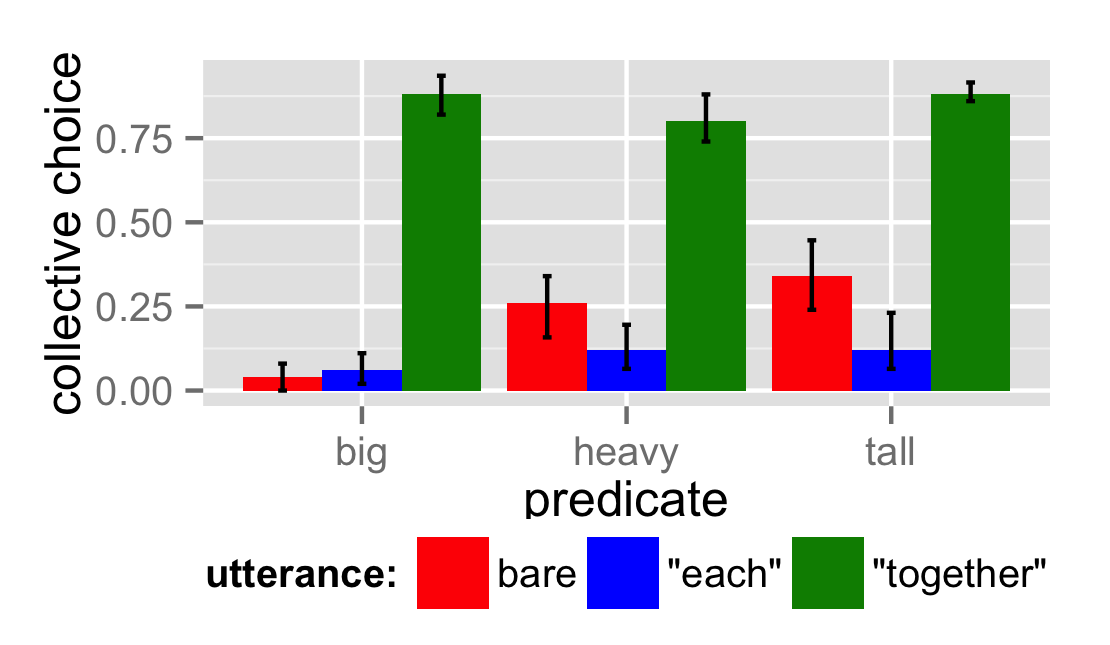
\includegraphics[width=\linewidth]{expt2.eps}}\\
	 	\vspace{-8pt}
	 	\mbox{Fig.~2: Expt.~1 collective response rate.}
	 \end{wrapfigure}
\textbf{Expt.~1 (N=50):} One way to access interpretations of ostensibly ambiguous plural predications is to elicit ratings of unambiguous paraphrases, for example rating \ref{each} and \ref{tog} as paraphrases of \ref{bare}. First, we must establish that these are in fact unambiguous paraphrases. To do so, we used a reference task.
Subjects were introduced to Cubert, an alien in a factory working with boxes. They were told that after receiving a shipment of boxes, Cubert told his friend Dot about them. The task was to help Dot decide which boxes Cubert was referring to; subjects chose between a collective interpretation-satisfying referent (Fig.~1, left) and a distributive interpretation-satisfying one (Fig.~1, right). Fig.~2 presents rates of collective referent choice for each of the three predicates and their three variants. The disambiguating paraphrases behave as expected: \emph{each} results in a distributive interpretation and \emph{together} results in collective. We also find that the bare form of \emph{big} patterns differently from \emph{heavy} and \emph{tall} -- it is more distributive. This finding is expected with respect to \textit{big} vs.~\textit{heavy}, but surprising given the behavior of \textit{tall}: both \emph{tall} and \emph{big} are size and shape predicates, so what allows \emph{tall} to more readily receive collective interpretations in our experimental context?  %Something beyond simply predicating properties of physical extent mediates the choice between distributive and collective interpretations. 
To identify this factor, consider first the difference between potentially collective and stubbornly distributive predicates.
Collective weight is a stable property of sets: regardless of the physical arrangement in which we encounter them, a set of boxes will have the same total weight. In other words, collective weight is contextually predictable. With collective height or size, these properties may change depending on physical arrangement: stacking boxes on top of each other or lining them up side by side, the total height of those boxes will change. With predicates of physical extent, collective properties are less contextually predictable when physical arrangements tend to vary. To communicate effectively and avoid possible confusion, collective interpretations should therefore be avoided. In other words, the more potential noise inherent to the collective interpretation of a predicate, the less useful and thus less likely that collective interpretation. Reducing noise to make the collective property more predictable on the basis of context, we should see collective interpretations become more available. In Expt.~2, we use the paraphrase methodology to investigate the role of contextual predictability.

%Consider \emph{heavy}, a predicate said to readily admit collective interpretations, and \emph{big}, a predicate said to resist them.  Here is a plausible explanation for stubborn distributivity. Language is used to communicate. Speakers aspire toward clarity in this process of communication. With a stubbornly distributive predicate, the collective property a speaker names (e.g., total size, length, width, etc.) might change depending on the arrangement of the things said to hold it. To communicate effectively and avoid possible confusion, collective interpretations should therefore be avoided; distributive interpretations are the safe bet. In other words, the more noise inherent to the collective interpretation of a predicate, the less likely that collective interpretation (and thus the more likely the distributive interpretation). If potential variability in the property being communicated influences the choice between distributive and collective interpretations, then manipulating contextual variability to decrease interpretation noise ought to make a collective interpretation more likely. Expt.~1 does just that.
 \begin{wrapfigure}[25]{r}{.5\textwidth}
 	\centering
 	\vspace{-10pt}
 	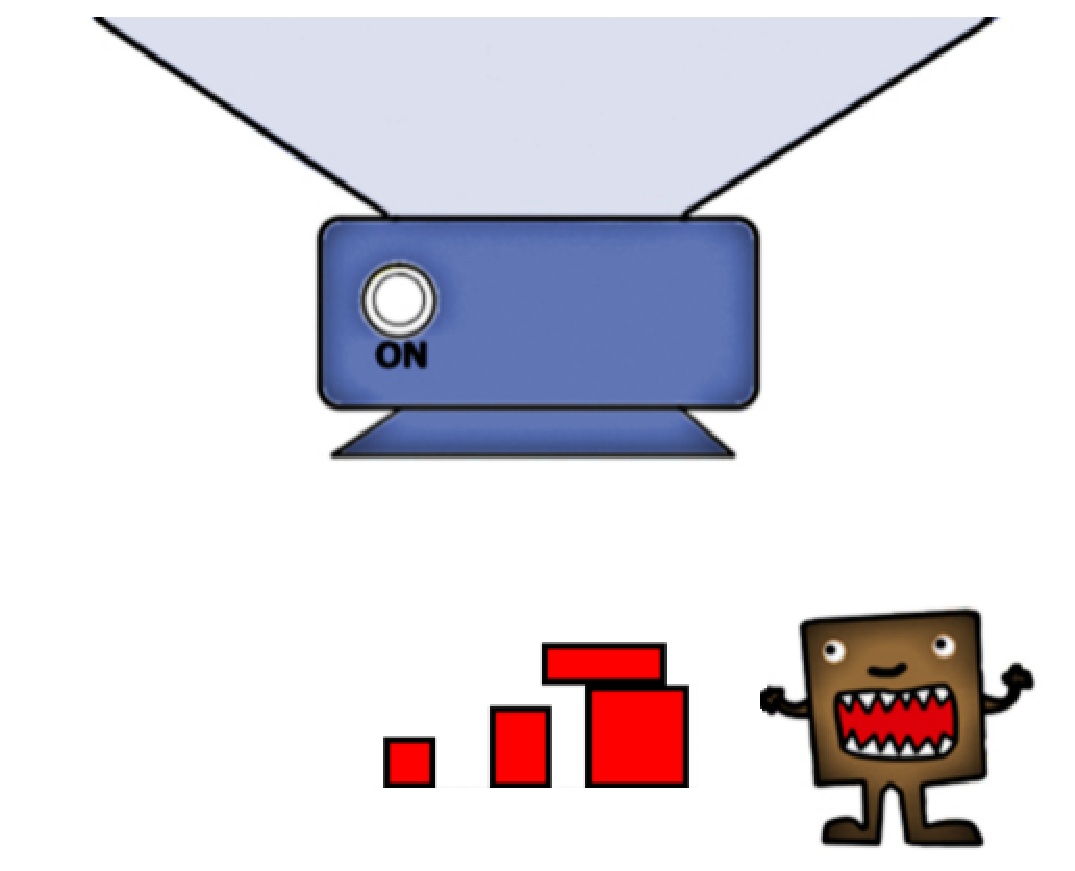
\includegraphics[width=.49\linewidth]{context13nodolly.eps}
 	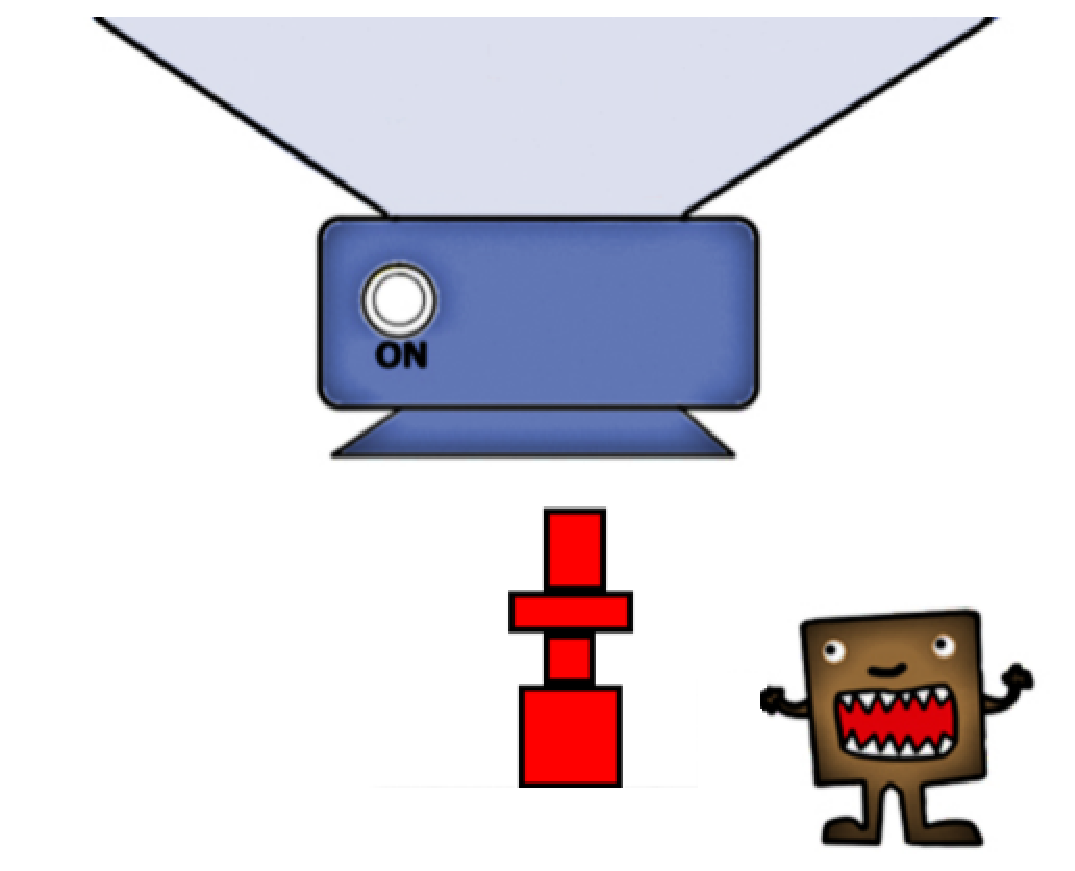
\includegraphics[width=.49\linewidth]{context13regnodolly.eps}\\
 	Fig.~3: Example context priming scenarios.\\[5pt]
 	\hspace{-5pt}\includegraphics[width=\linewidth]{trial1.eps}\\
 	Fig.~4: Example \emph{big} trial from Expt.~2.\\
 	\mbox{\hspace{-11pt}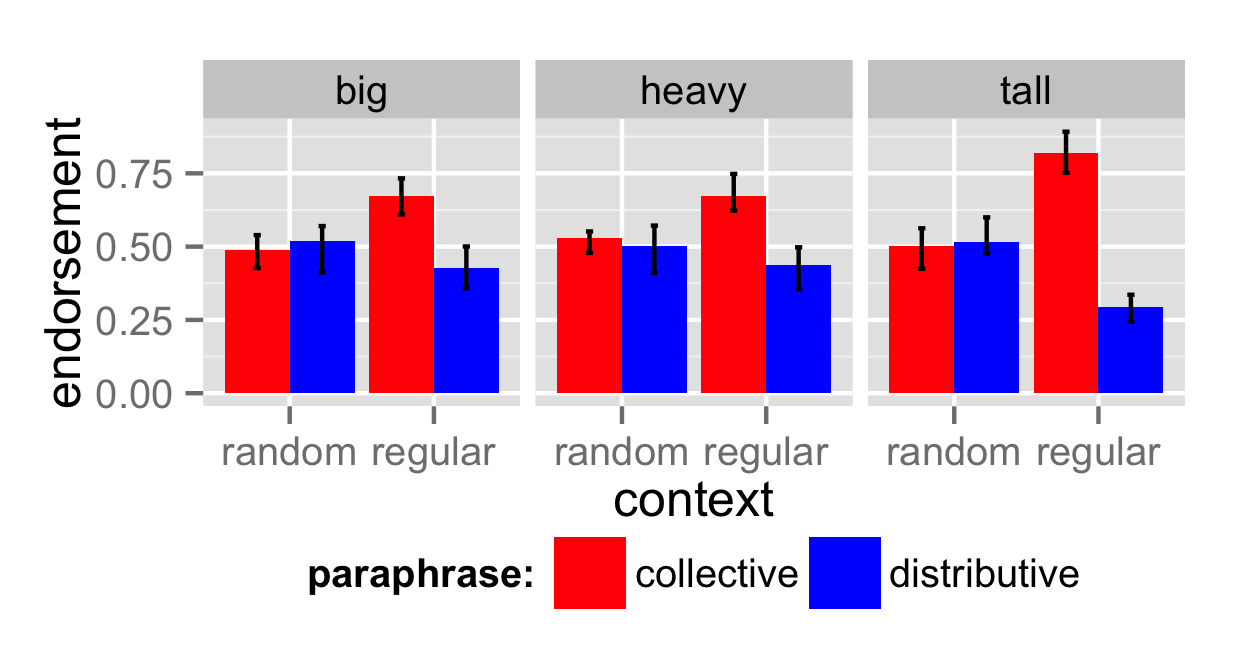
\includegraphics[width=.55\textwidth]{expt1.eps}}\\
 	\vspace{-8pt}
 	Fig.~5: Expt.~2 results.
 \end{wrapfigure}
\textbf{Expt.~2 (N=80):} If physical arrangements are less likely to change, collective predication becomes more predictable and stands a better chance of being informative. It should therefore become more likely. We manipulated predictability through a series of context scenarios. Subjects saw Cubert receive sets of boxes from a dispenser. Between subjects, the dispenser either dispensed boxes in \textsc{random} (Fig.~3, left) or \textsc{regular} physical arrangements (stacked on top of each other; Fig.~3, right). Subjects observed the dispenser four times, then Cubert spoke to his friend, Dot. Subjects were asked to help Dot understand Cubert's utterance by rating distributive and collective paraphrases on a sliding scale (Fig.~4). Fig.~5 presents average paraphrase endorsement rates for the three predicates tested. For each predicate, regular contexts had higher ratings for collective paraphrases and lower ratings for distributive. \textit{Tall} was most affected by our contextual manipulation, which directly targeted the height dimension, stacking boxes on top of each other. 

 Our results demonstrate the central role of context in plural predication: as collective properties become more predictable, collective interpretations become more viable, regardless of the predicate involved. We formalize this choice in a Bayesian RSA model \citep{frankgoodman2012,lassitergoodman2013}: noisy interpretations are less useful because they require more coordination between speakers and listeners; they are therefore less likely.

%These facts support a general model of rational communication under which the resolution of ambiguities is sensitive to the amount of variability in possible interpretations: A more variable interpretation is potentially less informative because it requires more coordination between speakers and listeners. The interpretation is therefore less likely.

		
% If sets of boxes regularly come stacked on top of each other, \textit{The boxes are big} is more likely to communicate that the total size of some set of boxes is large. These facts support a general model of rational communication under which the resolution of ambiguities is sensitive to the amount of variability in possible interpretations: A more variable interpretation is potentially less informative because it requires more coordination between speakers and listeners. The interpretation is therefore less likely.




\newpage

\bibliographystyle{chicago}
\bibliography{greg.bib}




\end{document}